% Provenance (never printed): see sources/outline_sources.md (Year 3:
% concordia and discordia; 40Ar/39Ar step heating; Sm-Nd model ages;
% cosmogenic nuclides; fission tracks and (U-Th)/He). Brief:
% sources/book5/BRIEFS.md, ch. 13. Curves from figdata/bachelor-3/
% concordia.py, arar_spectrum.py, model_ages.py, cosmogenic.py. Exercise and
% problem values in the Book 5 scratch calculator calc/ch13.py. The zircons,
% the biotite spectrum, the Nd sample and the helium ages of the Varden
% granite are invented, consistent with the Year 1 volume's granite of 310 Ma.
\chapter{Advanced Geochronology}\label{ch:b3:advanced-geochronology}

A crystal of zircon a tenth of a millimetre long has kept two clocks running
since its granite crystallised: uranium-238 decaying to lead-206 and
uranium-235 decaying to lead-207. When the two clocks agree, the age is
beyond doubt. When they disagree, the disagreement itself can be dated: the
crystal lost part of its lead in a later event, and the two clocks, read
together, give the age of the granite and the age of the event. This chapter
reads several clocks at once, in uranium and lead, in argon, in neodymium, in
fission tracks and helium, and in the rare atoms made by cosmic rays, and it
says how far each age can be trusted.

\begin{recall}
Radioactive decay, the age equation, the isochron and its initial ratio, the
least-squares line, branching decay, the potassium--argon age, closure
temperature and cooling age are in the Year 1 volume, in its chapter on
radiometric dating; the steady-erosion formula of \omterm{def:b3:advanced-geochronology:cosmogenic}{cosmogenic nuclides} is in
its chapter on erosion and transport. The chondritic uniform reservoir, the
epsilon notation and the depleted mantle are in the Year 2 volume, in its
chapter on isotope geochemistry; thermal ionisation and multi-collector mass
spectrometry in its chapter on field and lab methods. \omterm{def:b3:orogenic-wedges:thermochronology}{Thermochronology} and
the \omterm{def:b3:orogenic-wedges:age-elevation}{age--elevation relationship} are in \cref{ch:b3:orogenic-wedges}.
\end{recall}

\section{Uranium, lead and the concordia}\label{sec:b3:advanced-geochronology:upb}

Uranium has two long-lived isotopes. Uranium-238 decays through a chain of
short-lived daughters to lead-206 with $\lambda_{238} =
\qty{1.55125e-10}{yr^{-1}}$; uranium-235 decays to lead-207 with $\lambda_{235}
= \qty{9.8485e-10}{yr^{-1}}$, six times faster. Their present ratio is
$^{235}\mathrm{U}/^{238}\mathrm{U} = 0.0072567$, or $^{238}\mathrm{U}/^{235}\mathrm{U}
= 137.8$, the same in every terrestrial rock. Zircon, $\mathrm{ZrSiO_4}$, takes
in much uranium and almost no lead when it grows, and it resists weathering
and survives metamorphism: almost all its lead is radiogenic.
% ledger: amherst:constants, tulane:upb-zircon

Write $x = {}^{207}\mathrm{Pb}^*/{}^{235}\mathrm{U}$ and $y =
{}^{206}\mathrm{Pb}^*/{}^{238}\mathrm{U}$ for the present ratios of radiogenic
lead to its parent. Each gives an age, $t_{206} = \ln(1 + y)/\lambda_{238}$
and $t_{207} = \ln(1 + x)/\lambda_{235}$.

\begin{definition}[Concordia, discordia, intercepts, Tera--Wasserburg diagram]
\label{def:b3:advanced-geochronology:concordia}
The \emph{concordia}\index{concordia} is the curve of the $(x, y)$ plane on
which the two uranium--lead ages are equal. A \emph{discordia}\index{discordia}
is a straight line along which discordant analyses of one population of
crystals are aligned; its intersections with the concordia are the
\emph{upper intercept}\index{upper intercept} (the older) and the
\emph{lower intercept}\index{lower intercept} (the younger). The
\emph{Tera--Wasserburg diagram}\index{Tera--Wasserburg diagram} plots
$X = {}^{238}\mathrm{U}/{}^{206}\mathrm{Pb}^*$ against $Y =
{}^{207}\mathrm{Pb}^*/{}^{206}\mathrm{Pb}^*$.
\end{definition}

\begin{theorem}[The concordia]\label{thm:b3:advanced-geochronology:concordia}
A crystal that has stayed closed to uranium and lead since it formed, a time
$t$ ago, plots at
\[
C(t) = \bigl(e^{\lambda_{235}t} - 1,\; e^{\lambda_{238}t} - 1\bigr).
\]
As $t$ grows the curve rises ever more slowly against $x$: its slope,
$\mathrm dy/\mathrm dx = (\lambda_{238}/\lambda_{235})\,e^{(\lambda_{238} -
\lambda_{235})t}$, decreases from $\lambda_{238}/\lambda_{235} = 0.1575$ at the
origin, so the \omterm{def:b3:advanced-geochronology:concordia}{concordia} is concave towards the $x$ axis.
\end{theorem}

\begin{proof}
For each parent, the number of radiogenic daughters per parent atom left is
$e^{\lambda t} - 1$, the age equation of the Year 1 volume. Differentiating
both coordinates with respect to $t$ and dividing gives the slope; since
$\lambda_{235} > \lambda_{238}$, it decreases with $t$.
\end{proof}

Lead is a large ion that sits badly in the zircon lattice. In the parts of a
crystal damaged by its own radioactivity, it can leave in a later event of
heating or fluid circulation.
% ledger: tulane:upb-zircon

\begin{theorem}[Episodic lead loss gives a chord]\label{thm:b3:advanced-geochronology:discordia}
A crystal formed a time $t_1$ ago that lost, a time $t_2$ ago, a fraction $f$
of its radiogenic lead, and was closed otherwise, plots today at
\[
(1 - f)\,C(t_1) + f\,C(t_2),
\]
on the chord joining the points $t_1$ and $t_2$ of the \omterm{def:b3:advanced-geochronology:concordia}{concordia}. Crystals that
lost different fractions lie along that chord, a \omterm{def:b3:advanced-geochronology:concordia}{discordia} whose \omterm{def:b3:advanced-geochronology:concordia}{upper
intercept} is $t_1$ and \omterm{def:b3:advanced-geochronology:concordia}{lower intercept} is $t_2$.
\end{theorem}

\begin{proof}
Take one decay system, with constant $\lambda$, and count per atom of parent
present today. A time $t_2$ ago there were $e^{\lambda t_2}$ parent atoms, and
radiogenic daughters $e^{\lambda t_2}(e^{\lambda(t_1 - t_2)} - 1) =
e^{\lambda t_1} - e^{\lambda t_2}$. The event left $(1 - f)(e^{\lambda t_1} -
e^{\lambda t_2})$; since then the parent made $e^{\lambda t_2} - 1$ more. The
sum is $(1 - f)(e^{\lambda t_1} - 1) + f(e^{\lambda t_2} - 1)$. The two lead
isotopes behave alike chemically, so $f$ is the same for both, and the two
coordinates combine into the point stated.
\end{proof}

\begin{omfigure}
\begin{tikzpicture}
\begin{groupplot}[group style={group size=2 by 1, horizontal sep=1.7cm},
  omrecord, width=0.47\linewidth, height=0.42\linewidth, title style={font=\small},
  tick label style={font=\scriptsize}, label style={font=\small}]
\nextgroupplot[title={(a) concordia diagram},
  xlabel={$^{207}\mathrm{Pb}^*/^{235}\mathrm{U}$}, ylabel={$^{206}\mathrm{Pb}^*/^{238}\mathrm{U}$},
  xmin=0.04, xmax=0.44, ymin=0.006, ymax=0.06,
  xtick={0.1,0.2,0.3,0.4}, xticklabels={0.1,0.2,0.3,0.4},
  ytick={0.01,0.02,0.03,0.04,0.05}, yticklabels={0.01,0.02,0.03,0.04,0.05},
  scaled ticks=false]
% computed in figdata/bachelor-3/concordia.py
\addplot[black, thick] table[x=xw, y=yw] {figdata/out/bachelor-3-concordia-curve.dat};
\addplot[black, only marks, mark=*, mark size=1.4pt, nodes near coords={\scriptsize\pgfmathprintnumber[fixed, precision=0]{\pgfplotspointmeta}},
  point meta=explicit, nodes near coords align={anchor=south east},
  restrict expr to domain={\thisrow{t}}{100:350}]
  table[x=xw, y=yw, meta=t] {figdata/out/bachelor-3-concordia-ticks.dat};
\addplot[omDef, thick, densely dashed] table[x=x, y=y] {figdata/out/bachelor-3-concordia-line.dat};
\addplot[red!70!black, only marks, mark=diamond*, mark size=2pt] table[x=x, y=y] {figdata/out/bachelor-3-concordia-zircons.dat};
\nextgroupplot[title={(b) Tera--Wasserburg diagram},
  xlabel={$^{238}\mathrm{U}/^{206}\mathrm{Pb}^*$}, ylabel={$^{207}\mathrm{Pb}^*/^{206}\mathrm{Pb}^*$},
  xmin=15, xmax=75, ymin=0.0465, ymax=0.0535,
  ytick={0.047,0.049,0.051,0.053}, yticklabels={0.047,0.049,0.051,0.053},
  scaled ticks=false]
\addplot[black, thick] table[x=xtw, y=ytw] {figdata/out/bachelor-3-concordia-curve.dat};
\addplot[black, only marks, mark=*, mark size=1.4pt, nodes near coords={\scriptsize\pgfmathprintnumber[fixed, precision=0]{\pgfplotspointmeta}},
  point meta=explicit, nodes near coords align={anchor=north east},
  restrict expr to domain={\thisrow{t}}{100:250}]
  table[x=xtw, y=ytw, meta=t] {figdata/out/bachelor-3-concordia-ticks.dat};
\addplot[omDef, thick, densely dashed] table[x=xtw, y=ytw] {figdata/out/bachelor-3-concordia-twline.dat};
\addplot[red!70!black, only marks, mark=diamond*, mark size=2pt] table[x=xtw, y=ytw] {figdata/out/bachelor-3-concordia-zircons.dat};
\end{groupplot}
\end{tikzpicture}

\par\smallskip{\small (a) The \omterm{def:b3:advanced-geochronology:concordia}{concordia}, with its ages in millions of years,
and five invented discordant zircons of one granite (red; their error
ellipses are smaller than the symbols), aligned on a \omterm{def:b3:advanced-geochronology:concordia}{discordia} (dashed) that
meets the \omterm{def:b3:advanced-geochronology:concordia}{concordia} near 311 and \qty{100}{\Ma}. (b) The same zircons and line
in the \omterm{def:b3:advanced-geochronology:concordia}{Tera--Wasserburg diagram}, where a \omterm{def:b3:advanced-geochronology:concordia}{discordia} is still a straight
line.}\label{fig:b3:advanced-geochronology:concordia}
\end{omfigure}
% ledger: amherst:constants

The intercepts are found where $a + b\,x(t) = y(t)$, an equation in $t$ that is
solved by Newton's method: with $g(t) = e^{\lambda_{238}t} - 1 - a -
b(e^{\lambda_{235}t} - 1)$ and $g'(t) = \lambda_{238}e^{\lambda_{238}t} -
b\lambda_{235}e^{\lambda_{235}t}$, iterate $t \leftarrow t - g/g'$ from a guess
near each intercept. Three properties of the result matter in practice.
First, the \omterm{def:b3:advanced-geochronology:concordia}{upper intercept} is precise only if the \omterm{def:b3:advanced-geochronology:concordia}{discordia} crosses the
\omterm{def:b3:advanced-geochronology:concordia}{concordia} at a large angle. A young \omterm{def:b3:advanced-geochronology:concordia}{discordia}, as in the figure above, runs
almost along the \omterm{def:b3:advanced-geochronology:concordia}{concordia}, and a small change in its slope moves the
intercept far. Second, if the lead loss is recent, $t_2 = 0$, the \omterm{def:b3:advanced-geochronology:concordia}{discordia}
passes through the origin, and every crystal has the same
$^{207}\mathrm{Pb}^*/^{206}\mathrm{Pb}^*$ ratio,
\[
\frac{^{207}\mathrm{Pb}^*}{^{206}\mathrm{Pb}^*} = \frac{1}{137.8}\,
\frac{e^{\lambda_{235}t_1} - 1}{e^{\lambda_{238}t_1} - 1},
\]
which gives $t_1$ without the uranium: the lead--lead age. Third, a line in the
\omterm{def:b3:advanced-geochronology:concordia}{concordia} diagram, $x = (y - a)/b$, becomes in the Tera--Wasserburg
coordinates $Y = (1 - aX)/(137.8\,b)$, again a line. The \omterm{def:b3:advanced-geochronology:concordia}{Tera--Wasserburg
diagram} uses ratios measured directly, with no need to compute uranium-235
from uranium-238, and a mixture with common lead, unradiogenic and rich in
lead-207, plots on a line that reaches the $Y$ axis at the ratio of the common
lead.

Uranium--lead ages are measured in two ways. Single crystals or fragments,
dissolved after the damaged zones have been removed by partial dissolution
and their lead and uranium separated, are measured by thermal ionisation
mass spectrometry, with the most precise ages of geology. Spots a few tens of
micrometres across are measured in place, by an ion probe or by laser
ablation, less precisely but zone by zone through a crystal that grew in
several events.

\begin{inthelab}[The geochronology laboratory]
\begin{minipage}[t]{0.55\linewidth}\vspace{0pt}
A zircon date begins with a crushed rock and ends in a clean laboratory. The
geochronologists separate the zircons by density and magnetism, pick the
clearest crystals under the binocular microscope and image their zoning. The
crystals are partly dissolved to remove their damaged zones, then dissolved
completely with a spike of known isotopes, and the uranium and lead are
separated on tiny columns of resin, in air filtered to keep out the lead of
dust. A mass spectrometer measures the isotope ratios. Argon samples follow a
different path: a reactor, then a gas line where a laser heats each step and
the argon is cleaned before the spectrometer.
\end{minipage}\hfill
\begin{minipage}[t]{0.42\linewidth}\vspace{0pt}
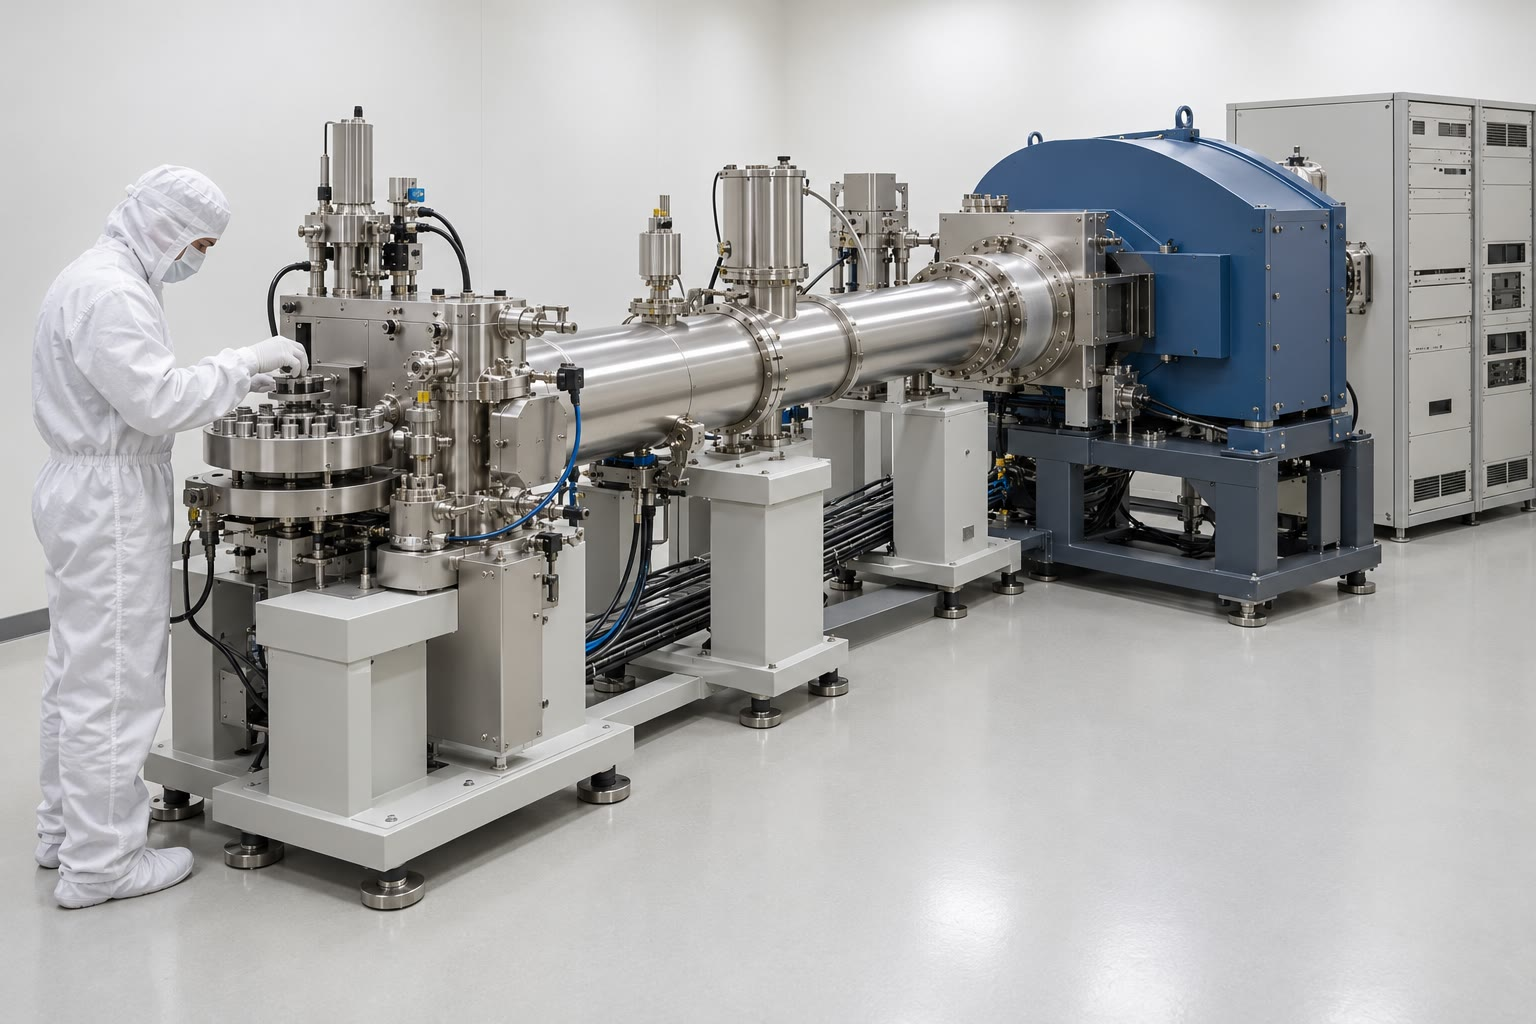
\includegraphics[width=\linewidth]{images/book5/ai/b3-mass-spec-lab.jpg}

{\scriptsize A mass spectrometer in a clean laboratory: the sample turret at
left, the flight tube and the electromagnet (AI-generated
illustration).}
\end{minipage}
\end{inthelab}

\section{Argon--argon dating}\label{sec:b3:advanced-geochronology:arar}

The potassium--argon method of the Year 1 volume measures the potassium and
the argon in two separate aliquots of a mineral. The argon--argon method
measures only argon, in one aliquot, as ratios of isotopes. The sample is
irradiated with fast neutrons in the core of a nuclear reactor, where the
reaction $^{39}\mathrm{K}(n,p)^{39}\mathrm{Ar}$ turns a fixed fraction of its
potassium-39 into argon-39, a proxy for potassium. A mineral of known age, the
monitor, is irradiated beside it.
% ledger: nmgrl:arar, amherst:arar

\begin{definition}[Argon--argon dating, J factor, age spectrum, plateau age]
\label{def:b3:advanced-geochronology:arar}
\emph{$^{40}\mathrm{Ar}/^{39}\mathrm{Ar}$ dating}\index{argon--argon dating@$^{40}\mathrm{Ar}/^{39}\mathrm{Ar}$ dating}
dates a potassium-bearing mineral by the ratio $R =
{}^{40}\mathrm{Ar}^*/{}^{39}\mathrm{Ar}_{\mathrm K}$ of its radiogenic argon-40
to the argon-39 made from its potassium by neutron irradiation. The
\emph{J factor}\index{J factor} of an irradiation is $J = (e^{\lambda
t_m} - 1)/R_m$, found from a monitor of known age $t_m$ and measured ratio
$R_m$, with $\lambda$ the total decay constant of potassium-40. When the sample
is degassed in steps of increasing temperature, its \emph{age
spectrum}\index{age spectrum} plots the age of each step against the
cumulative fraction of argon-39 released. A \emph{plateau
age}\index{plateau age} is the weighted mean age of consecutive steps that
agree within their uncertainties and release a large part of the argon-39.
\end{definition}

\begin{theorem}[The argon--argon age]\label{thm:b3:advanced-geochronology:arar}
A sample irradiated with a monitor has the age
\[
t = \frac1\lambda\ln(1 + JR).
\]
\end{theorem}

\begin{proof}
The radiogenic argon is $^{40}\mathrm{Ar}^* = (\lambda_e/\lambda)\,
{}^{40}\mathrm{K}\,(e^{\lambda t} - 1)$, by the branching decay of the Year 1
volume. The argon-39 made is $^{39}\mathrm{Ar}_{\mathrm K} =
{}^{39}\mathrm{K}\,\Phi$, where $\Phi$ collects the neutron dose and the
cross-section of the reaction. So $R = (e^{\lambda t} - 1)/J$ with $J =
\lambda\,\Phi\,{}^{39}\mathrm{K}/(\lambda_e\,{}^{40}\mathrm{K})$. The ratio
$^{40}\mathrm{K}/^{39}\mathrm{K}$ is the same in all potassium, and $\Phi$ the
same for two samples irradiated side by side, so $J$ is the same for the sample
and the monitor; the monitor's age and ratio give it, and inverting $R$ gives
$t$.
\end{proof}

The constants are those of the potassium--argon method, $\lambda =
\qty{5.543e-10}{yr^{-1}}$. A common monitor is a sanidine of a volcanic tuff
dated at \qty{28.201}{\Ma}; a monitor ratio $R_m = 1.3129$ gives $J =
0.01200$. Atmospheric argon, with $^{40}\mathrm{Ar}/^{36}\mathrm{Ar} = 295.5$,
is subtracted with the argon-36 measured in each step, and argon made by
neutrons from calcium and from potassium itself is corrected with salts
irradiated in the same package.
% ledger: schaen20:monitors, amherst:constants, nmgrl:arar

Step heating is the strength of the method. The sample is heated in a furnace
or by a laser in steps of increasing temperature, and each step gives an age.
If the mineral stayed closed since it cooled, all steps agree: the spectrum is
flat. If it lost argon from the rims of its grains, the first steps, which
come from the rims, are younger, and the ages rise as a staircase towards a
plateau given by the cores. The recommended criteria for a plateau are at
least five consecutive steps carrying more than \qty{50}{\percent} of the
argon-39, with no trend among them; the low-temperature steps of a staircase
are commonly read as a loss of radiogenic argon. Excess argon, trapped from a
fluid when the mineral grew, does the opposite: it makes some steps too old,
often the first and the last, in a saddle-shaped spectrum. The sum of all
steps, the total-gas age, is what a potassium--argon age would have given: an
average that hides the history.
% ledger: schaen20:plateau, nmgrl:arar

\begin{omfigure}
\begin{tikzpicture}
\begin{groupplot}[group style={group size=2 by 1, horizontal sep=1.5cm},
  omrecord, height=0.38\linewidth, title style={font=\small},
  xlabel={cumulative $^{39}\mathrm{Ar}$ released (\unit{\percent})},
  tick label style={font=\scriptsize}, label style={font=\small}]
\nextgroupplot[title={(a) the whole spectrum}, width=0.52\linewidth,
  ylabel={apparent age (\unit{\Ma})}, xmin=0, xmax=100, ymin=130, ymax=320,
  xtick={0,20,40,60,80,100}, ytick={150,200,250,300}]
% computed in figdata/bachelor-3/arar_spectrum.py
\addplot[omDef, thick] table[x=cum, y=age] {figdata/out/bachelor-3-arar_spectrum-boxes.dat};
\node[font=\scriptsize, anchor=west] at (axis cs:12,180) {argon loss};
\node[font=\scriptsize, anchor=north, red!70!black] at (axis cs:59,290) {plateau};
\nextgroupplot[title={(b) the plateau, enlarged}, width=0.44\linewidth,
  xmin=15, xmax=100, ymin=290, ymax=300, xtick={20,40,60,80,100},
  ytick={290,292,294,296,298,300}]
\addplot[name path=hi, draw=none, forget plot] table[x=cum, y=hi] {figdata/out/bachelor-3-arar_spectrum-boxes.dat};
\addplot[name path=lo, draw=none, forget plot] table[x=cum, y=lo] {figdata/out/bachelor-3-arar_spectrum-boxes.dat};
\addplot[omDef!25, forget plot] fill between[of=hi and lo];
\addplot[omDef, thick] table[x=cum, y=age] {figdata/out/bachelor-3-arar_spectrum-boxes.dat};
\draw[red!70!black, thick] (axis cs:18,296.1) -- (axis cs:100,296.1);
\node[font=\scriptsize, anchor=south, red!70!black] at (axis cs:59,290.3) {plateau \qty[separate-uncertainty=true]{296.1 \pm 0.8}{\Ma}};
\end{groupplot}
\end{tikzpicture}

\par\smallskip{\small The invented \omterm{def:b3:advanced-geochronology:arar}{age spectrum} of a biotite of the granite of
the first figure: each step is drawn at its age, its width the share of
argon-39 it released. (a) Three low-temperature steps rise as a staircase to a
plateau. (b) The seven plateau steps, which hold \qty{82}{\percent} of the
argon-39, with their two-standard-deviation ranges (shaded) and the \omterm{def:b3:advanced-geochronology:arar}{plateau
age} (red).}\label{fig:b3:advanced-geochronology:spectrum}
\end{omfigure}

\section{Neodymium model ages}\label{sec:b3:advanced-geochronology:model-age}

When a melt is extracted from the mantle to make continental crust, samarium,
more compatible, stays behind more than neodymium: the new crust has a lower
$^{147}\mathrm{Sm}/^{144}\mathrm{Nd}$ than its source, about 0.13 for most
crustal rocks, against 0.1966 for the chondritic reservoir. Its
$^{143}\mathrm{Nd}/^{144}\mathrm{Nd}$ then grows more slowly. Once formed, a
crustal rock tends to keep its samarium--neodymium ratio, through erosion,
sedimentation and even remelting, so its neodymium remembers when it left the
mantle.
% ledger: white08:model-age, white:chur

\begin{definition}[Model age]\label{def:b3:advanced-geochronology:model-age}
The \emph{model age}\index{model age} of a rock in an isotope system is the
time at which its ratio, projected back with its present parent--daughter
ratio, equals that of a model reservoir. For neodymium, $T_{\mathrm{CHUR}}$
uses the chondritic uniform reservoir and $T_{\mathrm{DM}}$ the depleted
mantle.
\end{definition}

\begin{theorem}[Model age]\label{thm:b3:advanced-geochronology:model-age}
A sample with present ratios $I_s = {}^{143}\mathrm{Nd}/^{144}\mathrm{Nd}$ and
$R_s = {}^{147}\mathrm{Sm}/^{144}\mathrm{Nd}$, compared with a reservoir of
present ratios $I_m$ and $R_m$, has the \omterm{def:b3:advanced-geochronology:model-age}{model age}
\[
T = \frac1\lambda\ln\left(1 + \frac{I_s - I_m}{R_s - R_m}\right),
\qquad \lambda = \lambda_{147}.
\]
\end{theorem}

\begin{proof}
A closed system had, a time $T$ ago, the ratio $I - R(e^{\lambda T} - 1)$: the
isochron equation read backwards. Equating this for the sample and the
reservoir gives $I_s - I_m = (R_s - R_m)(e^{\lambda T} - 1)$.
\end{proof}

With $\lambda_{147} = \qty{6.524e-12}{yr^{-1}}$, the reservoirs are the
chondritic one, 0.512638 and 0.1966 today, and the depleted mantle,
0.51315 today, about $\varepsilon_{\mathrm{Nd}} = +10$, which a closed
evolution from chondritic values since \qty{4.55}{\Ga} gives the ratio
$^{147}\mathrm{Sm}/^{144}\mathrm{Nd} = 0.2137$. An invented granite with
$I_s = 0.511900$ and $R_s = 0.1100$ has $\varepsilon_{\mathrm{Nd}} = -14.4$
today, $T_{\mathrm{CHUR}} = \qty{1.30}{\Ga}$ and $T_{\mathrm{DM}} =
\qty{1.84}{\Ga}$. The figure below reads both. The depleted-mantle age is the
better estimate, because the crust is extracted from a mantle already
depleted; it is the mean age at which the neodymium of the sample left the
mantle, its crustal residence age. Two caveats limit it: the crust must not
have changed its samarium--neodymium ratio since, and a rock made by mixing
old crust with new mantle melts has a meaningless intermediate \omterm{def:b3:advanced-geochronology:model-age}{model age}.
% ledger: villa20:sm147, white:chur, white08:model-age

\begin{omfigure}
\begin{tikzpicture}
\begin{axis}[omrecord, width=0.72\linewidth, height=0.38\linewidth,
  xlabel={time before present (\unit{\Ga})}, ylabel={$\varepsilon_{\mathrm{Nd}}$},
  xmin=0, xmax=2.5, ymin=-17, ymax=13, x dir=reverse,
  xtick={0,0.5,1,1.5,2,2.5}, xticklabels={0,0.5,1,1.5,2,2.5},
  tick label style={font=\scriptsize}, label style={font=\small},
  legend style={font=\scriptsize, at={(0.5,1.03)}, anchor=south, legend columns=3, legend cell align=left}]
% computed in figdata/bachelor-3/model_ages.py
\addplot[omDef, thick] table[x=t, y=eps_dm] {figdata/out/bachelor-3-model_ages-evolution.dat};
\addlegendentry{depleted mantle}
\addplot[black, thick, densely dashed] coordinates {(0,0) (2.5,0)};
\addlegendentry{CHUR}
\addplot[red!70!black, thick] table[x=t, y=eps_sample] {figdata/out/bachelor-3-model_ages-evolution.dat};
\addlegendentry{granite}
\draw[densely dotted] (axis cs:1.30,0) -- (axis cs:1.30,-17) node[above right, font=\scriptsize, rotate=90] {$T_{\mathrm{CHUR}}$};
\draw[densely dotted] (axis cs:1.84,5.4) -- (axis cs:1.84,-17) node[above right, font=\scriptsize, rotate=90] {$T_{\mathrm{DM}}$};
\end{axis}
\end{tikzpicture}

\par\smallskip{\small $\varepsilon_{\mathrm{Nd}}$ of an invented granite projected
back in time with its own samarium--neodymium ratio (red). It meets the
chondritic reservoir at $T_{\mathrm{CHUR}} = \qty{1.30}{\Ga}$ and the depleted
mantle (blue) at $T_{\mathrm{DM}} = \qty{1.84}{\Ga}$.}\label{fig:b3:advanced-geochronology:model-age}
\end{omfigure}

\section{Fission tracks and helium}\label{sec:b3:advanced-geochronology:low-t}

Uranium-238 also decays, very rarely, by spontaneous fission: the nucleus
splits into two fragments that fly apart and leave a trail of damage in the
crystal, up to \qty{9}{nm} wide and about \qty{23}{\micro\metre} long in
apatite. Etched with acid, the trails become visible under the microscope.
They heal when the crystal is heated, over about 20 to \qty{350}{\celsius}
depending on the mineral; in apatite, they shorten in the partial annealing
zone, about 60 to \qty{120}{\celsius}, and vanish above it.
% ledger: kohn24:ft, sueoka19:closure

\begin{definition}[Fission-track dating, track annealing]\label{def:b3:advanced-geochronology:fission-track}
\emph{Fission-track dating}\index{fission-track dating} dates a mineral by
the density of the tracks left in it by the spontaneous fission of
uranium-238, compared with its uranium content. \emph{Track
annealing}\index{track annealing} is the shortening and disappearance of the
tracks by repair of the crystal when it is heated.
\end{definition}

\begin{theorem}[The fission-track age]\label{thm:b3:advanced-geochronology:fission-track}
With $\lambda_f$ the decay constant of spontaneous fission and $\lambda =
\lambda_{238}$ the total one, a crystal with $N_s$ spontaneous fissions per unit
volume and $N$ atoms of uranium-238 has the age
\[
t = \frac1\lambda\ln\left(1 + \frac{\lambda}{\lambda_f}\,\frac{N_s}{N}\right).
\]
In the laboratory, the uranium is measured by inducing the fission of
uranium-235 with thermal neutrons, and the age becomes
\[
t = \frac1\lambda\ln\left(1 + \lambda\,\zeta\,g\,\rho_d\,\frac{\rho_s}{\rho_i}\right),
\]
with $\rho_s$ and $\rho_i$ the spontaneous and induced track densities,
$\rho_d$ the track density of a dosimeter glass, $g = 0.5$ a geometry factor
and $\zeta$ a calibration constant found on standards of known age.
\end{theorem}

\begin{proof}
Uranium-238 has decayed $N(e^{\lambda t} - 1)$ times, and the fraction
$\lambda_f/\lambda$ of these decays were fissions: $N_s =
(\lambda_f/\lambda)N(e^{\lambda t} - 1)$, which inverts into the first form.
The track densities are proportional to $N_s$ and to the number of induced
fissions, $N\,\sigma\,\Phi/137.8$, where $\sigma$ is the fission
cross-section of uranium-235 and $\Phi$ the neutron fluence, itself
proportional to $\rho_d$. The ratio $\rho_s/\rho_i$ is then $N_s/N$ times
a product of constants, and $\lambda_f$, $\sigma$, $137.8$ and the efficiency
of etching and counting are gathered with $g$ into $\zeta$.
\end{proof}

The fission decay constant is known only to within about \qty{10}{\percent},
between \num{7.9e-17} and \qty{8.7e-17}{yr^{-1}}, which is why most
laboratories prefer the $\zeta$ calibration. The lengths of the tracks keep
a record of the path in temperature. A rock that cooled fast through the
partial annealing zone has long tracks of nearly equal length; one that
lingered in it has shorter tracks of widely spread lengths, and the
fission-track age is then a mixed age, not the time of a passage through one
temperature.
% ledger: kohn24:ft

\begin{omfigure}
\begin{tikzpicture}[scale=0.85]
% (a) an etched apatite grain with tracks
\draw[thick, fill=omLithLime!15] (0,0) -- (3.2,0) -- (3.8,1.0) -- (3.2,2.0) -- (0,2.0) -- (-0.6,1.0) -- cycle;
\foreach \x/\y/\a in {0.4/0.5/30, 1.2/1.3/-20, 2.0/0.6/75, 2.6/1.4/10, 0.9/1.6/110, 1.7/0.9/150, 2.9/0.8/50}
  {\draw[very thick, black] (\x,\y) -- ++(\a:0.45);}
\node[font=\small] at (1.6,-0.4) {(a) etched tracks in apatite};
% (b) alpha ejection from a grain
\begin{scope}[xshift=6cm]
\draw[thick, fill=omLithLime!15] (0,0) rectangle (3.4,2.0);
\draw[dashed] (0.35,0.35) rectangle (3.05,1.65);
\fill[black] (0.2,1.0) circle (1.5pt) node[below right, font=\scriptsize] {U};
\draw[->, red!70!black, thick] (0.2,1.0) -- ++(160:0.7) node[left, font=\scriptsize] {He lost};
\fill[black] (1.7,1.0) circle (1.5pt);
\draw[->, red!70!black, thick] (1.7,1.0) -- ++(40:0.5);
\node[font=\scriptsize, align=center] at (1.7,0.55) {He kept};
\draw[<->] (3.05,1.8) -- (3.4,1.8) node[right, font=\scriptsize] {\qty{20}{\micro\metre}};
\node[font=\small] at (1.7,-0.4) {(b) alpha ejection};
\end{scope}
\end{tikzpicture}

\par\smallskip{\small Schematic. (a) Spontaneous fission tracks, revealed by
etching on a polished apatite grain, are counted per unit area. (b) An alpha
particle travels about \qty{20}{\micro\metre}: those emitted within that
distance of the surface (outside the dashed line) may leave the grain, so a
small grain keeps less of its helium.}\label{fig:b3:advanced-geochronology:low-t}
\end{omfigure}
% ledger: zeigler23:ejection

Each alpha decay emits a helium-4 nucleus. Uranium, thorium and their chains
accumulate helium in a crystal, which keeps it only when cool.

\begin{definition}[(U--Th)/He dating, partial retention zone]\label{def:b3:advanced-geochronology:uthhe}
\emph{(U--Th)/He dating}\index{U--Th/He dating@(U--Th)/He dating} dates a
mineral by the helium-4 accumulated from the alpha decays of uranium, thorium
and their daughters, compared with its uranium and thorium. The \emph{partial
retention zone}\index{partial retention zone} is the range of temperature in
which the helium produced is partly kept and partly lost by diffusion.
\end{definition}

\begin{theorem}[Helium ingrowth]\label{thm:b3:advanced-geochronology:helium}
A crystal closed to helium for a time $t$ holds
\[
\mathrm{He} = 8\,{}^{238}\mathrm U\,(e^{\lambda_{238}t} - 1)
+ 7\,{}^{235}\mathrm U\,(e^{\lambda_{235}t} - 1)
+ 6\,{}^{232}\mathrm{Th}\,(e^{\lambda_{232}t} - 1),
\]
in atoms, with the parents measured today; samarium-147 adds a small term.
\end{theorem}

\begin{proof}
Each chain loses its mass difference in alpha particles, four mass units each:
$(238 - 206)/4 = 8$, $(235 - 207)/4 = 7$, $(232 - 208)/4 = 6$, while beta
decays do not change the mass number. Each chain is at secular equilibrium,
so each parent decay is followed by its whole chain, and the number of
decays of each parent is that of the age equation.
\end{proof}

For a young crystal, $e^{\lambda t} - 1 \approx \lambda t$ and the age follows
from a single division. An alpha particle travels about
\qty{20}{\micro\metre} before it stops, so a crystal loses the helium made
near its surface; the measured age is divided by the retained fraction $F_T$,
which is smaller for small grains ($F_T = 0.70$ means \qty{30}{\percent}
lost). Apatite closes to helium at about 50 to \qty{80}{\celsius}, zircon at
160 to \qty{200}{\celsius}: with apatite fission tracks, near 90 to
\qty{120}{\celsius}, the low-temperature chronometers date the last few
kilometres of the ascent of a rock to the surface, as
\cref{ch:b3:orogenic-wedges} used them.
% ledger: zeigler23:ejection, sueoka19:closure, iaea:isotopes

\section{Cosmogenic nuclides}\label{sec:b3:advanced-geochronology:cosmogenic}

Cosmic rays striking the atmosphere make showers of secondary particles. The
fast neutrons that reach the ground break nuclei in the minerals of the top
metres of rock, by spallation: oxygen in quartz becomes beryllium-10, silicon
aluminium-26. Muons make some nuclides deeper, and dominate below about
\qty{3}{m}.
% ledger: zech04:exposure, portenga:method

\begin{definition}[Cosmogenic nuclide, exposure age, production rate]
\label{def:b3:advanced-geochronology:cosmogenic}
A \emph{cosmogenic nuclide}\index{cosmogenic nuclide} is a nuclide made in
a mineral at or near the surface by the secondary particles of cosmic rays. Its
\emph{production rate}\index{production rate (cosmogenic)} $P$ is the number
of atoms made per unit mass of mineral and per year. The \emph{exposure
age}\index{exposure age} of a surface is the time since it was first exposed
to cosmic rays, found from the concentration of a cosmogenic nuclide.
\end{definition}

The \omterm{def:b3:advanced-geochronology:cosmogenic}{production rate} decreases with depth as $P_0e^{-\rho z/\Lambda}$, where
the attenuation length is taken as $\Lambda = \qty{160}{g.cm^{-2}}$, about
\qty{60}{cm} of granite of density \qty{2.7}{g.cm^{-3}}. At the surface it
grows with altitude, because less air shields the rock, and with
geomagnetic latitude, because the field deflects fewer particles near the
poles. Rates are given for a reference at sea level and high latitude and
scaled to each site: one calibration gives $P_0 = \num{4.96}\text{ atoms}\,\unit{g^{-1}.yr^{-1}}$
of beryllium-10 in quartz at that reference. Beryllium-10 has a half-life of
\qty{1.388}{Myr}, $\lambda = \qty{4.994e-7}{yr^{-1}}$.
% ledger: balco08:params, zech04:exposure, lugaro:slr-table

\begin{theorem}[Exposure with decay and erosion]\label{thm:b3:advanced-geochronology:exposure}
A surface lowered at the steady rate $\varepsilon$, exposed for a time $t$
with no nuclide inherited, carries at its surface the concentration
\[
N(t) = \frac{P_0}{\mu}\bigl(1 - e^{-\mu t}\bigr), \qquad
\mu = \lambda + \frac{\rho\varepsilon}{\Lambda}.
\]
Without erosion, $N = (P_0/\lambda)(1 - e^{-\lambda t})$; after a long time,
$N = P_0/\mu$, and without decay this is the formula $P_0\Lambda/(\rho\varepsilon)$
of the Year 1 volume.
\end{theorem}

\begin{proof}
Follow the grain that is at the surface today. A time $s$ ago it was at the
depth $\varepsilon s$, where it gained atoms at the rate $P_0e^{-\rho\varepsilon
s/\Lambda}$; of those atoms the fraction $e^{-\lambda s}$ is left today. Summing
over the exposure,
\[
N = \int_0^t P_0e^{-\rho\varepsilon s/\Lambda}e^{-\lambda s}\,\mathrm ds
= \frac{P_0}{\mu}\bigl(1 - e^{-\mu t}\bigr).
\]
The limits follow by setting $\varepsilon = 0$, letting $t \to \infty$, and
then $\lambda = 0$.
\end{proof}

Without erosion the concentration saturates at $P_0/\lambda$ after a few
half-lives: a surface reaches \qty{90}{\percent} of it after $\ln 10/\lambda
= \qty{4.6}{Myr}$, and beyond that it can no longer be dated. With erosion,
the steady state is reached sooner, after a few times $1/\mu$, and its
concentration gives $\varepsilon$; the rate is averaged over the time
$\Lambda/(\rho\varepsilon)$ that the grain took to rise through one
attenuation length, a few tens of thousands of years at the rates of a few
tens of metres per million years. Outcrops of bedrock erode at a few metres
to a few tens of metres per million years; river basins, measured from the
sand of their rivers, faster.
% ledger: portenga:rates, portenga:method

Two nuclides with different half-lives date burial. Beryllium-10 and
aluminium-26 are made together in quartz in a fixed ratio; when a grain is
buried deep in a cave or under thick sediment, production stops, and
aluminium-26, which decays faster, falls behind: the ratio of the two decays
with time and dates the burial.

\section{The statistics of an age}\label{sec:b3:advanced-geochronology:statistics}

An age comes with its uncertainty, and a set of ages with the question
whether they agree. Let $n$ measurements $x_i$ of one quantity have standard
deviations $\sigma_i$. Their weighted mean is $\bar x = \sum w_ix_i/W$, with
$w_i = 1/\sigma_i^2$ and $W = \sum w_i$, and its standard deviation is
$1/\sqrt W$.

\begin{definition}[Mean square of weighted deviates]\label{def:b3:advanced-geochronology:mswd}
The \emph{mean square of weighted deviates}\index{mean square of weighted deviates}
(MSWD) of $n$ measurements about a fitted model with $p$ adjusted parameters
is
\[
\mathrm{MSWD} = \frac{1}{n - p}\sum_i \frac{(x_i - \hat x_i)^2}{\sigma_i^2},
\]
where $\hat x_i$ is the model value: $p = 1$ for a weighted mean, $p = 2$ for
a straight line such as an isochron or a \omterm{def:b3:advanced-geochronology:concordia}{discordia}.
\end{definition}

\begin{proposition}[The MSWD has expectation one]\label{prop:b3:advanced-geochronology:mswd}
If the $x_i$ are independent, normal, with the mean $\mu$ and the standard
deviations $\sigma_i$, the MSWD about their weighted mean has expectation 1.
\end{proposition}

\begin{proof}
Expanding $x_i - \mu = (x_i - \bar x) + (\bar x - \mu)$ and using $\sum
w_i(x_i - \bar x) = 0$,
\[
\sum w_i(x_i - \mu)^2 = \sum w_i(x_i - \bar x)^2 + W(\bar x - \mu)^2.
\]
On the left, each term has expectation 1, so the sum has expectation $n$. On
the right, $\bar x$ has variance $1/W$, so the last term has expectation 1.
Hence $\sum w_i(x_i - \bar x)^2$ has expectation $n - 1$.
\end{proof}

The MSWD scatters about 1 more widely when there are few degrees of freedom,
$f = n - p$: its upper limit at \qty{95}{\percent} is about $1 +
2\sqrt{2/f}$, 2.63 for $f = 3$ and 2.15 for $f = 6$. Above the limit, the
measurements scatter more than their uncertainties allow: the samples have
not all the same age, or the system was disturbed. Far below 1, the
uncertainties were overestimated.
% ledger: schaen20:mswd

\begin{method}[Fitting an isochron with errors on both axes]\label{met:b3:advanced-geochronology:york}
When both coordinates carry errors $\sigma_{x,i}$, $\sigma_{y,i}$, correlated
with the coefficient $r_i$, as in uranium--lead and isochron data:
\begin{enumerate}
\item start from the slope $b$ of the ordinary least-squares line;
\item give each point the weight $W_i = 1/(\sigma_{y,i}^2 + b^2\sigma_{x,i}^2 -
2br_i\sigma_{x,i}\sigma_{y,i})$, the inverse variance of its distance to the
line measured along $y$;
\item fit the weighted line with these weights, which gives a new $b$, and
return to step 2 until $b$ no longer changes;
\item compute the MSWD with the weights $W_i$ and $n - 2$ degrees of freedom,
and the uncertainty of the slope and intercept from the final weights.
\end{enumerate}
With $\sigma_{x,i} = 0$ the weights do not depend on $b$, and the method
reduces to the weighted least squares of $y$ on $x$ used in the problem.
\end{method}

The uncertainty of a decay constant is the same for every age of one system:
it does not enter when ages of one system are compared, but must be added
when ages from two systems are. The decay constant of samarium-147, for
instance, is known to about \qty{0.4}{\percent}; those of potassium-40,
branched and slow, limit the accuracy of argon ages.
% ledger: villa20:sm147, nmgrl:arar


\section{Exercises}

\begin{exercise}[$\star$]\label{exo:b3:advanced-geochronology:1}
A zircon has $^{206}\mathrm{Pb}^*/^{238}\mathrm{U} = 0.04500$ and
$^{207}\mathrm{Pb}^*/^{235}\mathrm{U} = 0.3300$. Compute its two
uranium--lead ages. Is it concordant? On which side of the \omterm{def:b3:advanced-geochronology:concordia}{concordia} does it
plot?
\end{exercise}
% ledger: amherst:constants

\begin{exercise}[$\star$]\label{exo:b3:advanced-geochronology:2}
A monitor of \qty{28.201}{\Ma} gives $R_m = 1.3129$. Compute $J$ with $\lambda
= \qty{5.543e-10}{yr^{-1}}$, then the age of a sample of the same irradiation
with $R = 10.000$ (use $J = 0.01200$).
\end{exercise}
% ledger: schaen20:monitors

\begin{exercise}[$\star$]\label{exo:b3:advanced-geochronology:3}
A shale has $^{143}\mathrm{Nd}/^{144}\mathrm{Nd} = 0.51180$ and
$^{147}\mathrm{Sm}/^{144}\mathrm{Nd} = 0.1200$. Compute its $T_{\mathrm{CHUR}}$
and $T_{\mathrm{DM}}$ with the values of the chapter.
\end{exercise}
% ledger: villa20:sm147, white:chur, white08:model-age

\begin{exercise}[$\star$]\label{exo:b3:advanced-geochronology:4}
A boulder of quartz on a moraine at the reference site holds \num{2.0e5}
atoms of beryllium-10 per gram. Assuming no erosion and no inheritance,
compute its \omterm{def:b3:advanced-geochronology:cosmogenic}{exposure age} without and then with decay, with $P_0 =
\num{4.96}\text{ atoms}\,\unit{g^{-1}.yr^{-1}}$.
\end{exercise}
% ledger: balco08:params, lugaro:slr-table

\begin{exercise}[$\star\star$]\label{exo:b3:advanced-geochronology:5}
Show that near the origin the \omterm{def:b3:advanced-geochronology:concordia}{concordia} is a line of slope
$\lambda_{238}/\lambda_{235}$, and compute it. Explain why the \omterm{def:b3:advanced-geochronology:concordia}{discordia} of
crystals that lost lead only very recently passes through the origin, and
what the lead--lead age of such crystals measures.
\end{exercise}

\begin{exercise}[$\star\star$]\label{exo:b3:advanced-geochronology:6}
Four step ages of a plateau are $296.4 \pm 0.8$, $295.1 \pm 1.0$, $297.0 \pm
0.9$ and \qty[separate-uncertainty=true]{295.8 \pm 0.7}{\Ma} ($1\sigma$). Compute their weighted mean,
its standard deviation and the MSWD. Do they agree?
\end{exercise}
% ledger: schaen20:mswd

\begin{exercise}[$\star\star$]\label{exo:b3:advanced-geochronology:7}
An apatite has $\rho_s = \qty{1.20e6}{cm^{-2}}$ and $\rho_i =
\qty{2.40e6}{cm^{-2}}$, with $\rho_d = \qty{1.10e6}{cm^{-2}}$, $g = 0.5$ and a
laboratory calibration $\zeta = \qty{350}{yr.cm^2}$. Compute its fission-track
age. What event does it date?
\end{exercise}
% ledger: kohn24:ft, sueoka19:closure

\begin{exercise}[$\star\star$]\label{exo:b3:advanced-geochronology:8}
An apatite holds \qty{20}{ppm} uranium (\qty{99.2742}{\percent}
uranium-238, \qty{0.7204}{\percent} uranium-235 by atoms), \qty{40}{ppm}
thorium-232 (half-life \qty{1.40e10}{yr}) and \qty{1.0}{nmol.g^{-1}} helium.
Compute its (U--Th)/He age with the linear approximation, then the age
corrected for alpha ejection with $F_T = 0.75$.
\end{exercise}
% ledger: iaea:isotopes, zeigler23:ejection

\begin{exercise}[$\star\star$]\label{exo:b3:advanced-geochronology:9}
For beryllium-10 at the reference site, compute the saturation concentration
without erosion and the time to reach \qty{90}{\percent} of it. Compute the
steady concentration of a surface eroding at \qty{10}{m.Myr^{-1}} (granite,
\qty{2.7}{g.cm^{-3}}, $\Lambda = \qty{160}{g.cm^{-2}}$).
\end{exercise}
% ledger: balco08:params, zech04:exposure, lugaro:slr-table

\begin{exercise}[$\star\star\star$]\label{exo:b3:advanced-geochronology:10}
Two measurements $x_1 \pm \sigma_1$ and $x_2 \pm \sigma_2$ of one age are
combined. Show that their MSWD about the weighted mean is
$(x_1 - x_2)^2/(\sigma_1^2 + \sigma_2^2)$, and prove directly that its
expectation is 1 when both measure the same age.
\end{exercise}

\begin{exercise}[$\star\star\star$]\label{exo:b3:advanced-geochronology:11}
A zircon of \qty{2700}{\Ma} lost lead at \qty{500}{\Ma} and has today
$^{206}\mathrm{Pb}^*/^{238}\mathrm{U} = 0.300$. What fraction of its lead did it
lose? Compute its $^{207}\mathrm{Pb}^*/^{235}\mathrm{U}$, its two uranium--lead
ages and, by iteration, its lead--lead age. Which of the three ages has a
meaning?
\end{exercise}

\begin{exercise}[$\star\star\star$]\label{exo:b3:advanced-geochronology:12}
A bedrock surface at the reference site holds \num{1.0e6} atoms of
beryllium-10 per gram. Compute its \omterm{def:b3:advanced-geochronology:cosmogenic}{exposure age} assuming no erosion, then its
erosion rate assuming a steady state. Show that every pair $(t, \varepsilon)$
between these two limits fits the measurement, and say what second
measurement would separate them.
\end{exercise}

\section{Problem: Zircons of the Varden Granite}

\begin{problem}[{Weekend problem --- the crystallisation, cooling and
unroofing of an invented granite, read on four clocks}]\label{pb:b3:advanced-geochronology:1}
The granite of the Varden Hills, the series' invented region, was unroofed
by the Triassic, buried under the Mesozoic cover and brought back to the
surface. Five of its zircons give, with one-standard-deviation errors on $y$
(take $x$ as exact):
\begin{center}
\small
\begin{tabular}{|l|ccccc|}
\hline
zircon & Z1 & Z2 & Z3 & Z4 & Z5 \\
\hline
$x = {}^{207}\mathrm{Pb}^*/^{235}\mathrm U$ & 0.3467 & 0.3260 & 0.3027 & 0.2793 & 0.2535 \\
$y = {}^{206}\mathrm{Pb}^*/^{238}\mathrm U$ & 0.04794 & 0.04505 & 0.04207 & 0.03892 & 0.03553 \\
$\sigma_y$ & 0.00010 & 0.00009 & 0.00008 & 0.00008 & 0.00007 \\
\hline
\end{tabular}
\end{center}
Use the constants of the chapter. All analyses are exercise data.
% ledger: amherst:constants, schaen20:monitors, schaen20:plateau, schaen20:mswd, sueoka19:closure, balco08:params, lugaro:slr-table

\medskip\noindent\textbf{Part I --- The zircons.}
\begin{enumerate}
\item Compute the two uranium--lead ages of each zircon. Are they concordant?
\item Why do the ages decrease from Z1 to Z5, with $t_{207} > t_{206}$ for
each?
\item Compute the Tera--Wasserburg coordinates of Z1 and Z5.
\item With the weights $w_i = 1/\sigma_{y,i}^2$, compute the weighted means
$\bar x$ and $\bar y$ and $S_{xx} = \sum w_i(x_i - \bar x)^2$.
\item Compute the slope $b = \sum w_i(x_i - \bar x)(y_i - \bar y)/S_{xx}$ and
the intercept $a$ of the \omterm{def:b3:advanced-geochronology:concordia}{discordia}.
\item Compare $b$ with the slope of the \omterm{def:b3:advanced-geochronology:concordia}{concordia} near \qty{310}{\Ma}. What
does this foretell?
\end{enumerate}

\medskip\noindent\textbf{Part II --- The intercepts.}
\begin{enumerate}[resume]
\item Find the \omterm{def:b3:advanced-geochronology:concordia}{upper intercept} by Newton's method from \qty{310}{\Ma}.
\item Find the \omterm{def:b3:advanced-geochronology:concordia}{lower intercept} from \qty{100}{\Ma}.
\item Compute the weighted residuals and the MSWD. Is the fit acceptable?
\item The standard deviation of the slope is $1/\sqrt{S_{xx}}$. Compute it.
\item Pivot the line about $(\bar x, \bar y)$ to the slopes $b \pm 2s_b$ and
recompute the \omterm{def:b3:advanced-geochronology:concordia}{upper intercept} for each. What is the uncertainty of the age?
\item What fraction of its lead did Z1 lose, and Z5?
\end{enumerate}

\medskip\noindent\textbf{Part III --- The biotite.} A biotite of the granite,
irradiated with a monitor of \qty{28.201}{\Ma} giving $R_m = 1.3129$, is
degassed in ten steps:
\begin{center}
\small
\begin{tabular}{|l|cccccccccc|}
\hline
step & 1 & 2 & 3 & 4 & 5 & 6 & 7 & 8 & 9 & 10 \\
$^{39}\mathrm{Ar}$ (\unit{\percent}) & 4 & 6 & 8 & 12 & 14 & 15 & 14 & 12 & 9 & 6 \\
$R$ & 7.225 & 11.226 & 13.937 & 14.891 & 14.820 & 14.869 & 14.918 & 14.847 & 14.907 & 14.804 \\
age (\unit{\Ma}) & & 228.0 & 279.0 & & 295.3 & 296.2 & 297.1 & 295.8 & 296.9 & \\
$\sigma$ (\unit{\Ma}) & 0.6 & 0.9 & 1.0 & 1.1 & 1.1 & 1.1 & 1.1 & 1.1 & 1.1 & 1.1 \\
\hline
\end{tabular}
\end{center}
\begin{enumerate}[resume]
\item Compute $J$; round it to 0.01200.
\item Compute the ages of steps 1, 4 and 10.
\item Which steps form a plateau by the criteria of the chapter?
\item Compute the \omterm{def:b3:advanced-geochronology:arar}{plateau age}, its standard deviation and its MSWD.
\item Compute the total-gas ratio and age. Why is it younger than the plateau?
\item Taking the granite to have crystallised at \qty{700}{\celsius} and the
biotite to close at \qty{375}{\celsius}, compute the mean cooling rate.
\item What could have happened at the \omterm{def:b3:advanced-geochronology:concordia}{lower intercept}? Is the argon spectrum
consistent with it?
\end{enumerate}

\medskip\noindent\textbf{Part IV --- The unroofing.} Four apatites, sampled
on a slope of the hills, give (U--Th)/He ages of 43.1, 46.0, 49.2 and
\qty{52.0}{\Ma} at 310, 370, 430 and \qty{490}{m}. The top of the granite,
on a gentle hill crest at a site where $P_0 = \num{5.6}\text{ atoms}\,\unit{g^{-1}.yr^{-1}}$,
holds \num{1.64e5} atoms of beryllium-10 per gram of quartz.
\begin{enumerate}[resume]
\item Compute the slope of the \omterm{def:b3:orogenic-wedges:age-elevation}{age--elevation relationship}, in metres per
million years.
\item With a closure temperature of \qty{65}{\celsius}, a surface at
\qty{10}{\celsius} and a geotherm of \qty{30}{\celsius.km^{-1}}, at what depth
did the lowest apatite close? What mean rate of unroofing since then follows?
\item Compute the present erosion rate from the beryllium-10, assuming a steady
state.
\item What rate does the formula of the Year 1 volume, without decay, give?
\item Over what time is the beryllium-10 rate averaged? Compare the three
rates.
\item State the age of crystallisation of the Varden granite with its
uncertainty.
\end{enumerate}
\end{problem}
